Una delle euristiche più utilizzate per risolvere il \ddbpp{} è la \emph{bottom-left} (BL), che consiste nel prendere uno ad uno in un certo ordine i pacchetti da inserire nel bin e farli cadere il più in basso possibile per poi spostarli più a sinistra possibile, trovando una posizione valida quando il pacchetto appoggia su una superficie sia a sinistra che in basso. Questa euristica è particolarmente importante in quanto è stato dimostrato che se esiste un modo per disporre un certo insieme di pacchetti in un \emph{bin} esiste anche una permutazione dell'insieme che permette di inserire tali pacchetti nel suddetto bin tramite l'euristica BL. Prendendo quindi un \emph{bin} delle dimensioni minime per contenere la soluzione ottima è possibile dimostrare che questa è ottenibile tramite l'algoritmo BL.

L'algoritmo BL in media però non è molto efficiente in quanto può lasciare degli spazi vuoti che se vengono chiusi da un pacchetto non possono più essere utilizzati nei passi successivi dell'algoritmo. Per risolvere questo problema è stata ideata la variante Bottom-Left-Fill (BLF) che consiste nell'inserire ogni pacchetto nella posizione più in basso possibile considerando anche le posizioni all'interno dei buchi lasciati dal placing dei pacchetti precedenti. A parità di altezza vengono privilegiate le posizioni più a sinistra. Il BLF si presta bene all'utilizzo combinato con algoritmi genetici in quanto associa una permutazione dei pacchetti ad un particolare placing degli stessi e garantisce che almeno una delle permutazione conduca ad un placing ottimo. Si può perciò pensare di utilizzare come cromosoma una sequenza ordinata di pacchetti (eventualmente ruotati) ed applicare ad essa mutazioni e cross-over order-based per giungere ad una soluzione di fitness massima.

Pur essendo un'euristica molto semplice a livello intuitivo, l'implementazione naive di questo algoritmo richiede tempo $O(n^4)$ nel numero di pacchetti, in questo progetto invece abbiamo deciso di utilizzare l'implementazione proposta da Chazelle \cite{chazelleBL} che richiede spazio lineare e tempo $O(n^2)$ nel numero di pacchetti. In questa sezione verrà descritta l'idea alla base dell'algoritmo ideato da Chazelle e le nostre scelte implementative. 

\subsection{Descrizione dell'algoritmo}
Ad ogni stadio dell'algoritmo BLF, ogni \emph{bin} contiene degli spazi vuoti detti \emph{hole}, che possono essere visti come poligoni formati da solo lati orizzontali e verticali. L'algoritmo procede esaminando uno alla volta gli \emph{hole} e determinando tutte le posizioni in cui può essere inserito il rettangolo corrente, per poi scegliere la posizione più in basso a sinistra. Ogni hole viene rappresentato con una lista dei suoi lati. Un lato di un hole viene detto \emph{leftmost edge} se forma, con i due lati ad esso adiacenti, due angoli convessi ed entrambi i due lati giacciono alla sua destra. Al contrario, un lato di un hole viene detto un \emph{notch} se forma, con i due lati ad esso adiacenti, due angoli concavi. Un \emph{notch} verticale in particolare viene detto \emph{left notch} se i due lati ad esso adiacenti giacciono alla sua sinistra. Infine, un angolo concavo con al di sopra un lato verticale e un lato orizzontale alla sua destra viene detto \emph{falling corner}.
Per prima cosa, per ogni hole bisogna individuare tutti i \emph{left notch} e i \emph{leftmost edge} ad essi associati e suddividere l'\emph{hole} nei relativi \emph{sub-hole} nel modo rappresentato in figura \ref{fig:imgBLF1}.

\begin{figure}[h!tp]
 \centering
 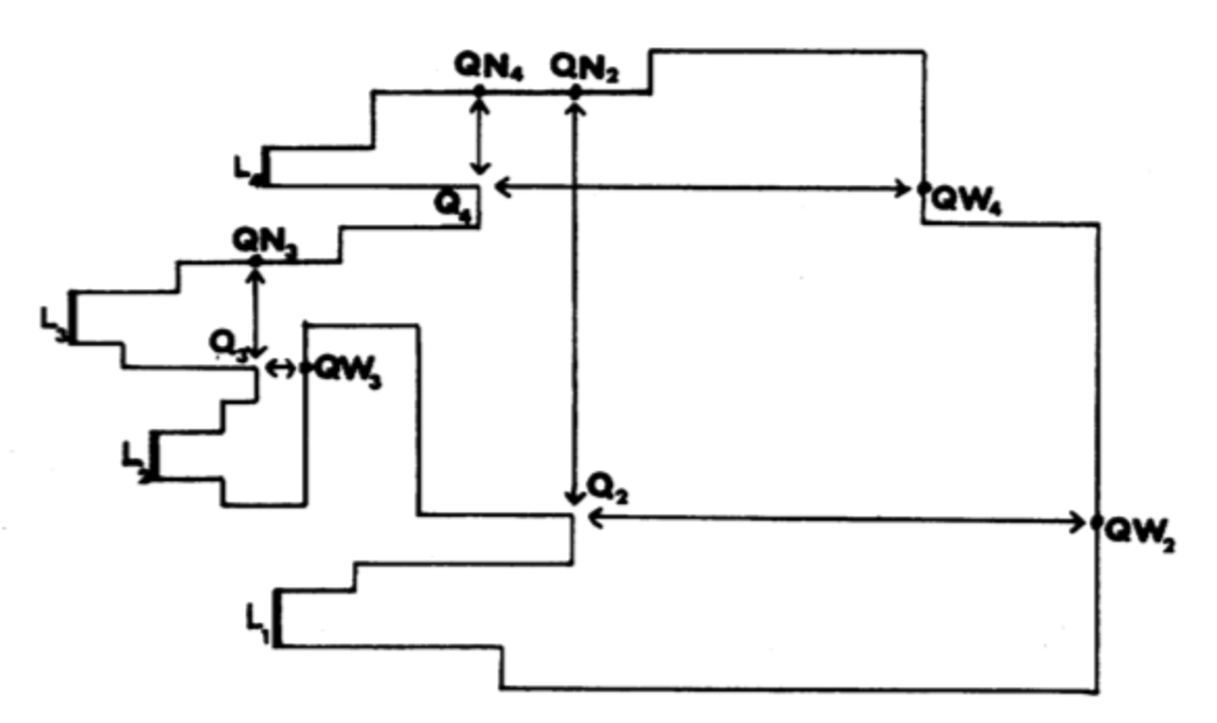
\includegraphics[width=0.8\textwidth]{./img/imgBLF1.pdf}
 % imgBLF1.pdf: 584x347 pixel, 72dpi, 20.60x12.24 cm, bb=0 0 584 347
 \caption{Individuazione dei \emph{left notches} e \emph{leftmost edge} associati.}
 \label{fig:imgBLF1}
\end{figure}

Si può dimostrare che ognuno di questi \emph{sub-hole} è \emph{nice} cioè non contiene left, right o upper \emph{notch} e contiene al massimo un \emph{falling corner}. Una volta ottenuti dei \emph{sub-hole} di questo tipo, possiamo, in tempo lineare, trovare tutte le posizioni dove può essere inserito il pacchetto all'interno del \emph{sub-hole}.
Definiamo $FB$ la lista dei punti che delimitano la parte inferiore del \emph{sub-hole} ed $FT$ quella dei punti che ne delimitano la parte superiore. 
Per prima cosa pensiamo di rimuovere la \emph{linea poligonale} corrispondente ad $FT$, ottenendo quindi un area $A$ infinita delimitata inferiormente da $FB$. Consideriamo ora un segmento $(b1,b2)$ di lunghezza pari a quella del rettangolo da inserire. Dobbiamo trovare tramite la procedura \texttt{Bottom}, l'insieme dei punti $C$ tali che, $p \in C$ se, considerando la verticale dove giace $p$, esso è il punto $b1$ con coordinata $y$ minima tale che il segmento $(b1,b2)$ giace interamente nell'area $A$.
Consideriamo ora l'area $B$ infinita, delimitata superiormente da $FT$ e troviamo l'insieme dei punti $D$ di coordinata $y$ massima tali che il segmento sia contenuto interamente in $B$. Questi due insiemi possono essere trovati in tempo lineare scorrendo le relative liste $FB$ e $FT$.

\begin{figure}[h!tp]
 \centering
 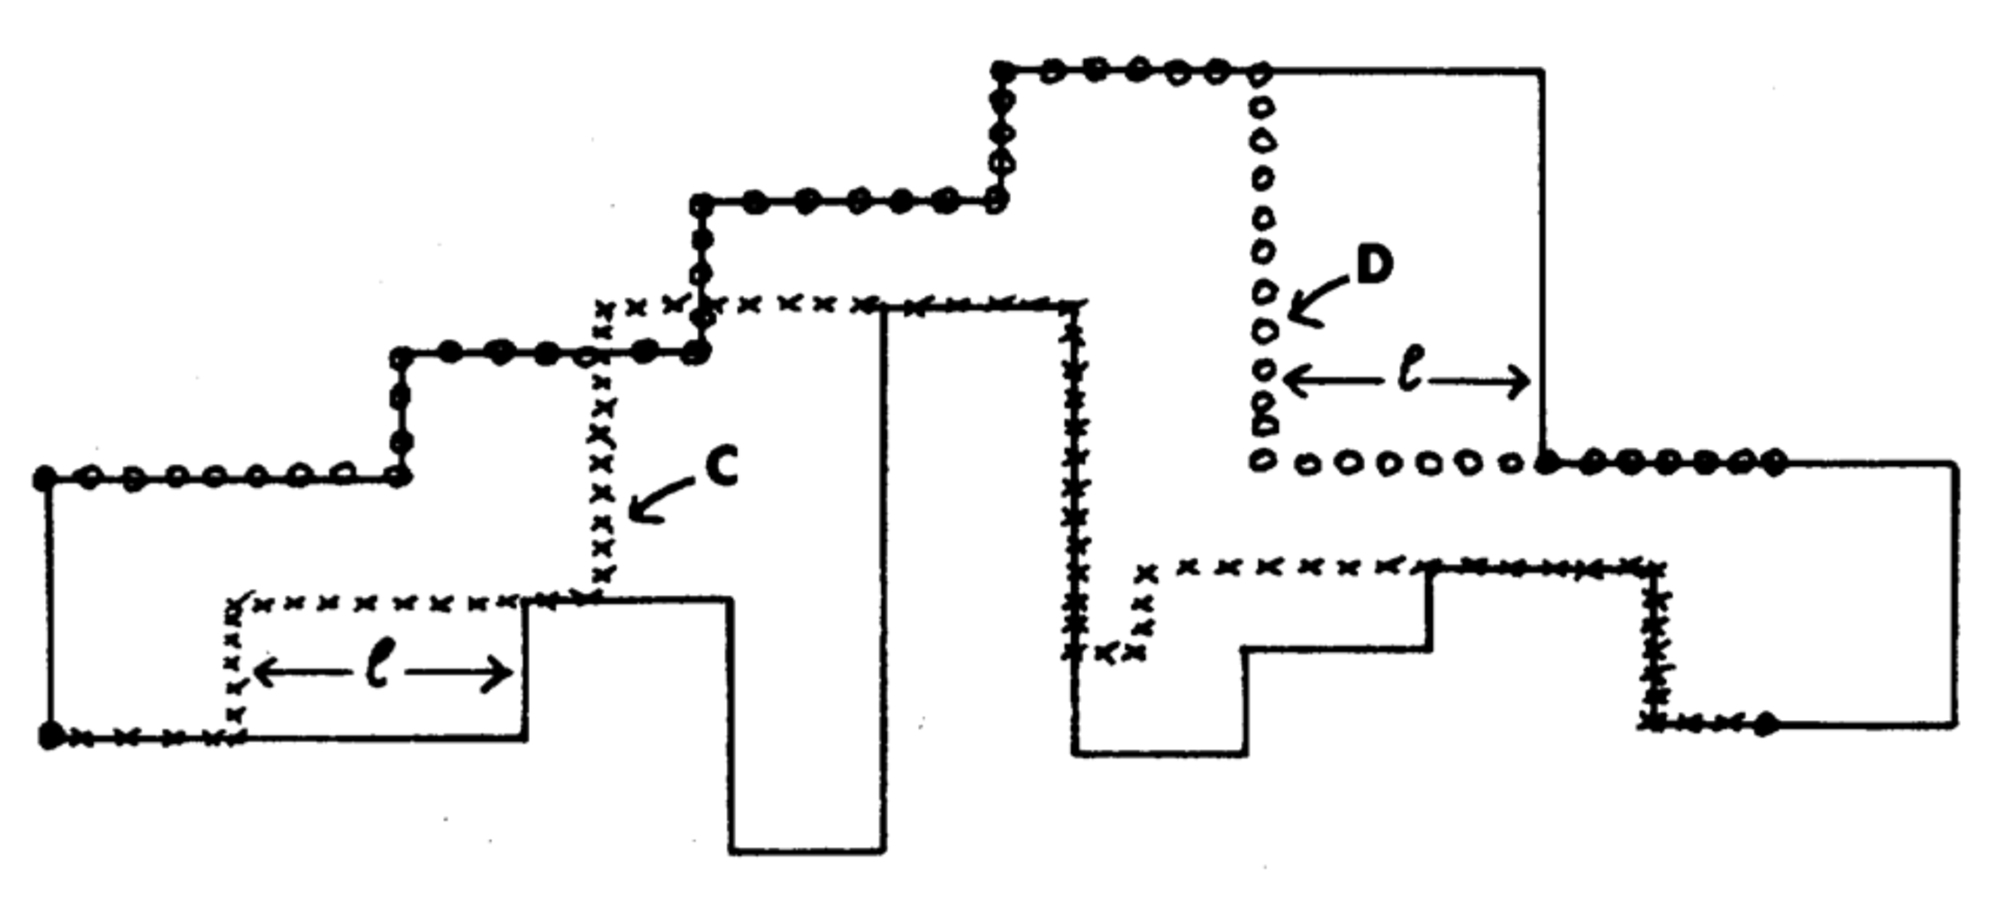
\includegraphics[width=0.8\textwidth]{./img/imgBLF2.pdf}
 % imgBLF2.pdf: 962x432 pixel, 72dpi, 33.94x15.24 cm, bb=0 0 962 432
 \caption{}
 \label{fig:imgBLF2}
\end{figure}

A questo punto, per trovare i punti dove è possibile inserire il rettangolo basta scorrere da sinistra a destra contemporaneamente i due insiemi e riportare come feasible i punti di $C$ tali che la differenza di altezza con il punto di $D$ nella stessa verticale sia maggiore dell'altezza del rettangolo. Il tutto può essere eseguito ancora una volta in tempo lineare nel numero di pacchetti già inseriti. L'algoritmo che inserisce uno alla volta tutti i pacchetti risulterà quindi essere di complessità $O(n^2)$.